\begin{enquestion}{20}{
    A military research team is evaluating the relationship between the weight of a battle tank and the time it takes to deploy the vehicle in combat situations (in hours).
    The team collects the following data on 10 different vehicles:
    {\par\bigskip
        \begin{center}
            \begin{tabular}{c|cccccccccc}
                \toprule
                    \textbf{Vehicle weight (in tons)} & $5$ & $6$ & $7$ & $8$ & $9$ & $10$ & $11$ & $12$ & $13$ & $14$ \\
                \midrule
                    \textbf{Deployment time (hours)} & $4.2$ & $4.8$ & $5.1$ & $5.3$ & $5.9$ & $6.0$ & $6.7$ & $6.8$ & $7.2$ & $7.4$ \\
                \bottomrule
            \end{tabular}
        \end{center}
    \par\bigskip}
    The research team believes that there is a linear relationship between the weight of the vehicle and the deployment time.
}

    \subquestion{4}{
        Draw a scatter plot based on the sample given above.
        Please indicate explicitly for both axes which variable it represents.
    }
    \ensolution{
        The $x$-axis indicates the independent variable, in this case the weight of the vehicle in tons.

        The $y$-axis indicates the dependent variable, in this case the deployment time in hours.\rubric{2}
        \begin{center}
            \resizebox{\textwidth}{!}{
                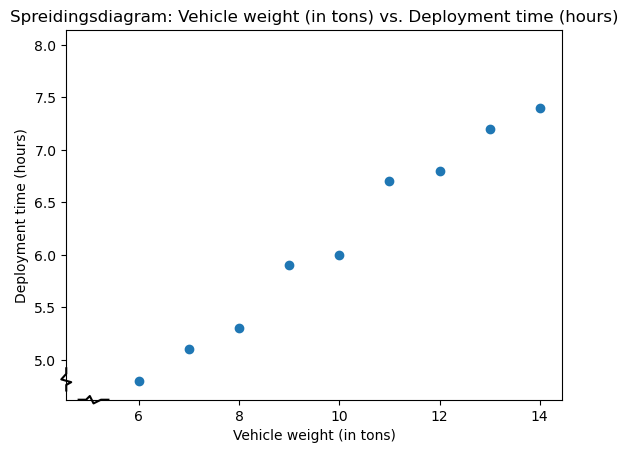
\includegraphics{exam20261204-scatterplot.png} \rubric{2}
            }
        \end{center}
    }
    
    \subquestion{8}{
        Calculate the least-squares estimate of the regression line $Y = \beta_0 + \beta_1 X$.
    }

    \ensolution{
        We start by generating a table based on the data, the sample sums and means can then be used to calculate the least-squares estimated $\hat{\beta}_0$ and $\hat{\beta}_{1}$:
        \begin{center}
            \begin{tabular}{ccccc}
            	\toprule
            		$X$ & $Y$ & $XY$ & $X^2$ & $Y^2$ \\
            	\midrule
            		$5$ & $4.2$ & $21.0$ & $25$ & $17.64$ \\ 
            		$6$ & $4.8$ & $28.8$ & $36$ & $23.04$ \\ 
            		$7$ & $5.1$ & $35.7$ & $49$ & $26.01$ \\ 
            		$8$ & $5.3$ & $42.4$ & $64$ & $28.09$ \\ 
            		$9$ & $5.9$ & $53.1$ & $81$ & $34.81$ \\ 
            		$10$ & $6.0$ & $60.0$ & $100$ & $36.0$ \\ 
            		$11$ & $6.7$ & $73.7$ & $121$ & $44.89$ \\ 
            		$12$ & $6.8$ & $81.6$ & $144$ & $46.24$ \\ 
            		$13$ & $7.2$ & $93.6$ & $169$ & $51.84$ \\ 
            		$14$ & $7.4$ & $103.6$ & $196$ & $54.76$ \\ 
            	\midrule
            		$\sum X = 95$ & $\sum Y = 59.4$ & $\sum XY = 593.5$ & $\sum X^2 = 985$ & $\sum Y^2 = 363.32$ \\ 
            		$\overline{X} = 9.5$ & $\overline{Y} = 5.94$ & $\overline{XY} = 59.35$ & $\overline{X^2} = 98.5$ & $\overline{Y^2} = 36.332$ \rubric{3} \\ 
            	\bottomrule
            \end{tabular}
        \end{center}
        
        
        Using the standard formulas for the least-squares estimates, we get
        \begin{align*}
            \hat{\beta}_1 &= \frac{\overline{xy} - \overline{x} \cdot \overline{y}}{\overline{x^2} - (\overline{x})^2} \\
              &= \frac{59.3500 - 9.5000 \cdot 5.9400}{98.5000 - (9.5000)^2} \\
              &= \frac{2.9200}{8.2500} \approx 0.3539 \rubric{2} \\
            \hat{\beta}_0 &= \overline{y} - \hat{\beta}_1 \cdot \overline{x} \\
              &= 5.9400 - 0.3539 \cdot 9.5000 \\
              &\approx 2.5776. \rubric{2}
        \end{align*}        
        The equation of the regression line is thus equal to $Y = 2.5776 + 0.3539X$. \points{1}
    }
    
    \subquestion{3}{
        Interpret the slope $\beta_{1}$ of the regression model in the context of this exercise. 
        What does the slope suggest about the relationship between vehicle weight and deployment time?
    }

    \ensolution{
        In the context of this question, the slope $\beta_{1}$ of the regression tells us how much more time it takes to deploy a vehicle in combat situations if the weight of the vehicle increases (by one ton). \rubric{1}

        Since the least-squares estimate $\hat{\beta}_1$ of the slope is positive, this suggests that the deployment time increases whenever the vehicle weight increases. \rubric{2}
    }

    \subquestion{5}{
        Calculate the correlation coefficient $r(x,y)$ between the vehicle weight and deployment time. 
        Based on the value of the correlation coefficient, what can you conclude about the strength and direction of the relationship between the two variables?}

    \ensolution{
        The correlation coefficient $r(x,y)$ can be computed as follows:
        \begin{align*}
            r(x,y) = \frac{\Cov{x}{y}}{\sqrt{s_{X}^2\cdot s_{Y}^2}} &= \frac{\sum_{i=1}^n x_iy_i - n \cdot \overline{x} \cdot \overline{y}}{\sqrt{(\sum_{i=1}^n x_{i}^2 - n \cdot \overline{x}^2) \cdot (\sum_{i=1}^n y_{i}^2 - n \cdot \overline{y}^2)}}   \\
            &= \frac{593.5 - 10 \cdot 9.5 \cdot 5.94}{\sqrt{(985 - 10 \cdot 9.5^2) \cdot (363.32 - 10 \cdot 5.94^2)}} \\
            &\approx 0.9929 \rubric{3}
        \end{align*}
        
        The value of the correlation coefficient is very close to 1, which suggests a very strong positive correlation between vehicle weight and deployment time in a combat situation. \rubric{2}
    }
\end{enquestion}